\section{Problemlösungsverfahren und Systemarchitektur}
\label{sec:architecture}

Ausgehend von der Literaturbesprechung in \autoref{sec:literatur} sowie den Schlussfolgerungen zur Farbgestaltung von Webseiten in \autoref{sec:farbgestaltung} wird im Folgenden eine Methode zur Problemlösung besprochen. Darauf aufbauend wird in \autoref{sec:architektur} die konkrete Architektur des zu implementierenden Systems vorgestellt.

\subsection{Regelbasierter oder probabilistischer Ansatz}
\label{sec:ansatz}

\citet{webpage} stellen für die automatisierte Farbgestaltung zwei grundlegende Herangehensweisen vor:

\begin{enumerate}
	\item \textbf{Regelbasiert:} Beschreibt quantitative Modelle mit determinstischem Regelwerk. Die Arbeit von \citet{magazines} zur automatisierten Färbung von Magazincovern stellt hierfür ein Beispiel dar. Durch die Analyse von Farbharmonie-Modellen wurden Regeln für Farbbeziehungen abgeleitet.
	\item \textbf{Datengetrieben:} Beschreibt Modelle, welche die Performanz möglicher Lösungen einer automatisierten Farbgestaltung auf Grundlage existierender Beispieldaten vorhersagt.
\end{enumerate}

Die regelbasierten Modelle treffen strickte Aussagen auf einem gewissen Abstraktionsgrad durch eine Vereinfachung des Problems bis zu einer Ebene, auf der Entscheidungen auf Grundlage weniger Parameter getroffen werden (z.B. durch die Angabe fester Grenzwerte). Im Gegensatz dazu stützen sich die Modelle des datengetriebenen Ansatzes auf reale Beispiele und tendieren daher zu robusteren Ergebnissen in der Anwendungsdomäne \citep{webpage}. Durch die Vielfalt der Beispieldaten findet ein verstärkter Einsatz probabilistischer Modelle statt \citep[siehe z.B.][]{webpage, patterns}.

Da bei probabilistischen Modellen alle potentiellen Lösungen bewertet und gegeneinander abgewogen werden müssen, sind hohe Laufzeiten möglich. Die bereits entwickelte Lösung von \citet{webpage} zur automatisierten Farbgestaltung von Webseiten benötigt selbst nach einer Optimierung des Suchverfahrens, bei der unwahrscheinliche Lösungen frühzeitig ausgeschlossen werden, bis zu 2 Stunden zur Konvergenz. Darüber hinaus ist deren vorgestellter Prozess zur Anpassung der Farbgestaltung einer Webseite an eine Bildvorlage nicht im eigentlichen Sinne automatisiert: Einerseits erfordert die Verwendung des K-Means Algorithmus zur CPE die Eingabe der Farbanzahl ($k$) vom Gestalter, andererseits erfordert die lexikographische Strategie einen Nutzerinteraktion während des Optimierungsprozesses.

Aus diesen Gründen wird sich in dieser Arbeit für eine vollautomatisierte, regelbasierte Lösungsmethode entschieden. Auch ohne die Auswertung großer Datenmengen existieren quantitative Modelle zur Gewährleistung der Textlesbarkeit und Benutzerführung, wie z.B. die in \ref{sec:lesbarkeit} vorgestellten quantitativen Grenzwerte der \emph{Web Content Accessibility Guidelines}.

\subsection{Layouts}
\label{sec:layouts}

Ziel dieser Arbeit die Färbung eines konkreten Webseite. Das Parsing eines solchen HTML-Dokuments zur Erschließung aller $e \in CG$ sowie die Speicherung aller topologischen Informationen dieser Elemente innerhalb einer Seite führt jedoch eine zusätzliche Ebene der Komplexität in das zu lösende Problem ein. Der CSS-Standard sieht durch die Klassen-Selektoren \citep{css3-selectors} ohnehin die Auszeichnung einheitlicher darzustellender Elemente bereits auf Ebene der Dokumentenbeschreibung vor. Dementsprechend wird von der konkreten HTML-Beschreibung einer Webseite als  \textbf{Layout} abstrahiert. Ein Layout definiert:

\begin{enumerate}
	\item $FGs$: Die Menge der $k$ Funktionsgruppen $FGs$. Entsprechend \autoref{sec:farbgestaltung} wird diese standardmäßig auf $FGs = \{\text{Primär}, \text{Sekundär}, \text{Akzent}, \text{Interaktion}, \text{Text (neutral)}, \text{Hintergrund (neutral)}\}$ festgelegt.
	\item $CGs$: Die Menge der Color Groups mit den enthaltenen Elementen $CGs = \{CG_1 = (e_1, e_2, ...), ..., CG_m = (e_1, e_2, ...)\}$.
 	\item $CGs \to FGs$: Die Abbildung der Color Groups auf Funktionsgruppen. Beispielsweise definiert ein Layout selbst, welche Elementen interaktiv sind und somit zur Farbfunktion \emph{Interaktion} gehören.
\end{enumerate}

Somit wird die Komplexität der Suchverfahren reduziert, indem die Menge der Funktionsgruppen als konstant angesehen wird und die konkrete Topologie der Oberflächenelemente innerhalb des HTML-Dokuments im Verantwortungsbereich des Layouts liegt.

\subsection{Aufteilung der Suchverfahren}
\label{sec:aufteilung}

Formale stellt sich die automatisierte Farbgestaltung einer Webseite aus einer Bildvorlage als die Abbildung $f_\text{coloration}: (CPs \to FGs) \to (I \to P)$ dar. In \autoref{sec:layouts} wurde dargestellt, dass zur Lösungssuche die Ermittlung der Abbildung $CGs \to FGs$ als gegeben durch das Layout angesehen und somit aus der Betrachtung entfernt wird. Weiterhin existieren die Teilprobleme (1) $f_{CPE}: I \to P$, d.h. die Ermittlung von $n$ repräsentativen Farben einer Bildvorlage sowie (2) Die Ermittlung des Farbschemas $f_\text{scheme}: FGs \to P$, d.h. die Auswahl von $k$ Farben aus der Palette und deren Zuordnung zu den Funktionsgruppen.

In \autoref{sec:architektur} wurde ein regelbasierter Ansatz zur Lösungssuche gewählt. Die Regeln werden im Folgenden als \textbf{Constraints} bezeichnet. Es existieren zwei Herangehensweisen:
\begin{enumerate}
    \item \textbf{Constraints-First}: Setze $|FGs| = k = n = |P|$. $P$ wird in Abhängigkeit vom Layout ermittelt. Hierbei wird die Ermittlung des Farbschemas zum Zeitpunkt der CPE verlagert. Unter Kenntnis der Funktionsgruppen mit deren gewünschten Eigenschaften ist der Suchraum das Histogram der Bildvorlage. Dieser Ansatz wird unter anderem von \citet{colorcomp} verfolgt. Sie verwenden ihr Regressionsmodell zur Bewertung der Farbharmonie, um eine alternative Optimierungsfunktionen zur Suche von $P$ im Farbraum einer Bildvorlage zu formulieren.
    \item \textbf{Constraints-Last}: Setze $k \leq n$. $P$ wird unabhängig vom Layout ermittelt. Der Suchraum für das Farbschema beschränkt sich auf die Farben in $P$. Dieser Ansatz wird ebenfalls von \citep{webpage} bei der datengetriebenen Färbung von Webseiten verfolgt.
\end{enumerate}

Für diese Arbeit wird die Herangehensweise \textbf{Constraints-Last} bevorzugt, um Flexibilität in Bezug auf unterschiedliche Layouts zu gewährleisten. Für die Arbeit bedeutet dies, dass eine Problemlösung anhand eines exemplarischen Layouts mit einer definierten Menge an Funktionsgruppen veranschaulicht wird, eine Übertragung auf andere Layouts jedoch möglich ist.

Selbst unter den gegebenen Einschränkung des Suchraums durch die vorgeschaltete Ermittlung einer Farbpalette ist die Menge potentieller Lösungen mit $\binom{n}{k} k!$ nach wie vor groß. Als Beispiel sei ein Layout mit 5 Funktionsgruppen sowie eine Farbpalette mit 10 Farben gegeben. Somit gilt $|FGs| = k = 5$ und $|P| = n = 10$, wodurch sich $\binom{10}{5} 5! = 30.240$ mögliche Kombinationen ergeben. Dementsprechend ist ein effektives Suchverfahren für die Ermittlung des Farbschemas zu ermitteln. Die von \citet{patterns} verwendeten Factor Graphs stellen hierfür einen Ansatz dar.

\subsection{Systemarchitektur}
\label{sec:architektur}

\begin{figure}
	\centering
	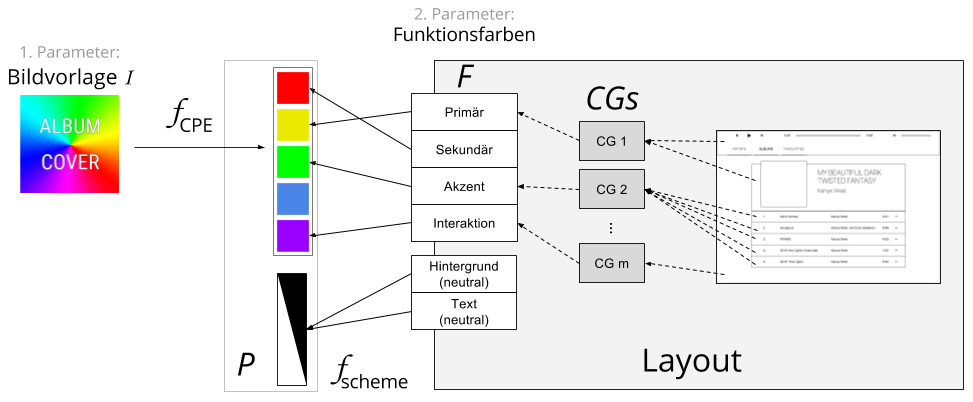
\includegraphics[width=1\textwidth]{img/architecture.png}
	\caption{System-Architektur. Der grau unterlegte Kasten visualisiert den Bereich, für den algorithmische Lösungen gefunden werden müssen. Die Eingabeparameter sind eine Bildvorlage und eine Menge von Color Groups, welche von einem Layout definiert werden. Das System setzt zwei Suchverfahren um, welche mit $f1$ und $f2$ bezeichnet werden. $f1$ ermittelt zuerst eine Farbpalette aus der Bildvorlage (CPE). $f2$ ordnet Colour Groups Farben aus der Palette, in dem ein entsprechendes Constraint System gelöst wird. Nachdem eine Farbabbildung gefunden wurde, wird das kolorierte Layout ausgegeben.}
	\label{fig:architecture}
\end{figure}

Abbildung \ref{fig:architecture} fasst die Systemarchitektur für die die automatisierte Farbgestaltung einer Webseite zusammen. Parameter 1 ist die Bildvorlage \emph{I}, welche durch einen Algorithmus zur Color Palette Estimation $f_{CPE}$ auf eine Menge repräsentativer Farben abgebildet wird. Aus \autoref{sec:usability} folgt, dass unabhängig von der Bildvorlage Weiß und Schwarz für den neutralen Text bzw. Hintergrund benötigt werden. Darum wird die Farbpalette um die in \autoref{sec:lesbarkeit} genannten Werte ergänzt, $P = f_{CPE}(I) \cup \{rgba(255, 255, 255, 1.0), rgba(0, 0, 0, .87)\}$

Parameter 2 sind die Funktionsgruppen, welche in \autoref{sec:funktionsgruppen} festgelegt wurden. Durch ein Suchverfahren $f_\text{scheme}$ werden Farben für die einzelnen Funktionsgruppen gesucht, d.h. es wird ein Farbschema gebildet. Hierfür wird ein Constraint System Modelliert und durch die von \citet{patterns} vorgestellten Factor Graphs implementiert.

